\chapter{Empirical Results}\label{chap:mainresults}
\todo{chapter intro} The approach usually starts with the problem definition and continues with what you have done. Try to give an intuition first and describe everything with words and then be more formal like `Let $g$ be ...'.

Start with a very short motivation why this is important. Then, as stated above, describe the problem with words before getting formal.
\section{Database}

The data used for this study is from the tick-by-tick Trade and Quote database traded at the NYSE. As \citet{hausman1992} use one-year data for their analysis, we also take the full trading sample of IBM stock on NYSE from January 3 to December 29 of 2023 for the descriptive statistics and market microstructure analysis parts. For the forecasting analysis, the first 10 months of 2023 will be used for in-sample forecasting, and the last 2 months will be left for the out-of-sample forecasting.

Before arriving at the final dataset, we first match the trade and quote databases. Since the resolution of the current NYSE database is at nanosecond, we simply backward match the trade to the prevailing quote. We only use the data within the regular trading hours (9:30:00–16:00:00) and do not take into account overnight trading. The transactions happening at the first-second of each trading day are removed to reduce contamination from the opening call at the stock exchange. \tabref{tab:table-2} summarizes the number of observations used:

\begin{table}[ht]
\centering
\small
\renewcommand{\arraystretch}{1.3} % Increases row height
\setlength{\tabcolsep}{10pt} % Increases column separation
\resizebox{\textwidth}{!}{%
\begin{tabular}{|c|l|c|}
\hline
\textbf{Purpose}       & \multicolumn{1}{c|}{\textbf{Timeframe}} & \textbf{Number of transactions} \\ \hline
Panel A: Total         & January 3 - December 29, 2023           & 1,905,393                       \\ \hline
Panel B: In-sample     & January 3 - October 31, 2023            & 1,641,694 (86\% of total sample) \\ \hline
Panel B: Out-of-sample & November 1 - December 29, 2023          & 263,699 (14\% of total sample)   \\ \hline
\end{tabular}%
}
\caption{Summary of Database: IBM traded on NYSE, 2023}
\label{tab:table-2}
\end{table}


\section{Descriptive Statistics (Full Sample)}

{\noindent\bfseries Price Change }

\figref{fig:price-change-2023} depicts the histogram of transaction price changes for IBM on NYSE in 2023 by \textit{tick }(equivalent to \$0.01 or 1 cent). The distribution of price changes seems to be almost symmetric around zero, which is expected for a very liquid stock like IBM. Moreover, the histogram shows that the majority of mass lies in the range of -4 to +4-tick changes. In order to also account for more extreme cases, we could choose the number of state \textit{m} = 14, including the changes from <-6 to >+6-tick. 




\begin{figure}[htbp]
    \centering
    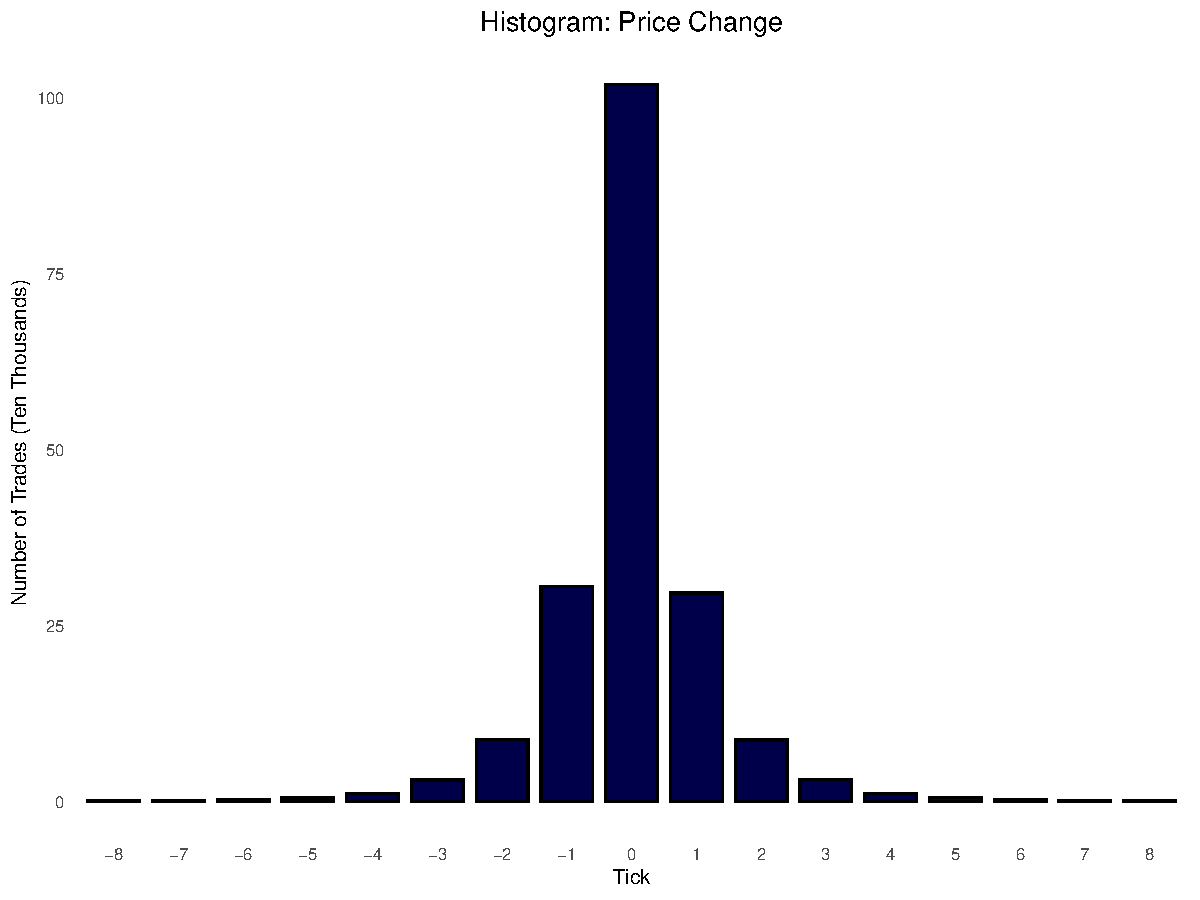
\includegraphics[width=0.8\textwidth]{figures/descriptive stat/price_change_IBM_N_2023.pdf}
    \caption{Histogram of Price Changes: IBM on NYSE, 2023}
    \label{fig:price-change-2023}
\end{figure}







\begin{table}[h]
  \centering
  \setlength{\tabcolsep}{4pt} 
  \resizebox{\textwidth}{!}{%
    \begin{tabular}{@{} r *{14}{r} @{}}
      \toprule
      \textbf{Category}      & 1    & 2       & 3       & 4       & 5       & 6       & 7       & 8       & 9       & 10   
      & 11      & 12      & 13      & 14      \\
      
      \textbf{Price Changes}   & <–6  & [–6,–5) & [–5,–4) & [–4,–3) & [–3,–2) & [–2,–1) & [–1,0)  & [0,1)   & [1,2)   & [2,3)   & [3,4)   & [4,5)   & [5,6)   & \geq6     \\
    
      \textbf{Percentage} & 0.31\% & 0.16\%   & 0.33\%   & 1.83\%   & 2.68\%   & 8.18\%   & 11.08\%  & 62.00\%  & 7.99\%   & 2.68\%   & 1.89\%   & 0.34\%   & 0.17\%   & 0.34\%  \\
      \bottomrule
    \end{tabular}%
  }
  \caption{Frequencies of Partition (Price Changes in Ticks)}
  \label{tab:table-3}
\end{table}

Besides, most of the trade occurs at either higher than or lower than mid-quote prices as similar to the results of \citet{hausman1992} or \citet{kim2014}.

\begin{table}[H]
\centering
\resizebox{0.25\textwidth}{!}{%
\begin{tabular}{ll}
\toprule
\textbf{\% trades at prices} & \\
> Midquote & 40.07\\
= Midquote & 16.65\\
< Midquote & 43.28\\
\textbf{Price change, $Z_k$} & \\
Mean & 0.0000\\
Std. dev. & 0.0134\\
\bottomrule
\end{tabular}}
\caption{Summary statistics: Price Changes}
\label{tab:table-4}
\end{table}



{\noindent\bfseries Trade Direction }

As mentioned in the previous chapter, the trade direction is determined via the procedure proposed by \citet{leeready1991} that incorporates two major steps. Firstly, the trade price is compared with the mid-quote to see if it is greater than mid-quote then it is buyer-initiated trade and vice versa, hereby noted as "mid-quote rule". Secondly, in case the price is equal to the mid-quote then a "tick-test" is applied. The "tick-test" will then compare the current trade with the previous trade's price. If there is again no difference between the two consecutive price then the sign of the last non-zero change will be selected. \citet{hausman1992} adopts only the "mid-quote rule" and thus has the third classification of "indeterminate" trade $IBS = 0$. If we would use the same procedure, our buyer-initiated classfication would simply be the percentage of trade with price > mid-quote (i.e. 40.07\%), and seller-initiated classification would be 43.28\%. Hence, our final results showed in \tabref{tab:table-5} with roughly similar proportion (48.43\% buyer-initiated versus 51.57\% seller-initiated) are reasonable.


\begin{table}[H]
\centering
\resizebox{0.4\textwidth}{!}{%
\begin{tabular}{lr}
\toprule
\textbf{Trade direction, $IBS_k$ }& \\
Buyer-initiated (\%) & 48.43\\
Seller-initiated (\%) & 51.57\\
Mean & -0.0313\\
Std. dev. & 0.9995\\
\bottomrule
\end{tabular}}
\caption{Summary statistics: Trade Direction}
\label{tab:table-5}
\end{table}

{\noindent\bfseries Other Variables }


\section{Panel A: Market Microstructure Analysis}

\section{Panel B: Forecasting Analysis}